\documentclass[../PHYS306Notes.tex]{subfiles}

\begin{document}
\section{Lecture 10}
\subsection{Lecture Notes - Intro to Coupled Oscillators}
\subsubsection{Analysis with Newtonian Mechanics}
\begin{center}
    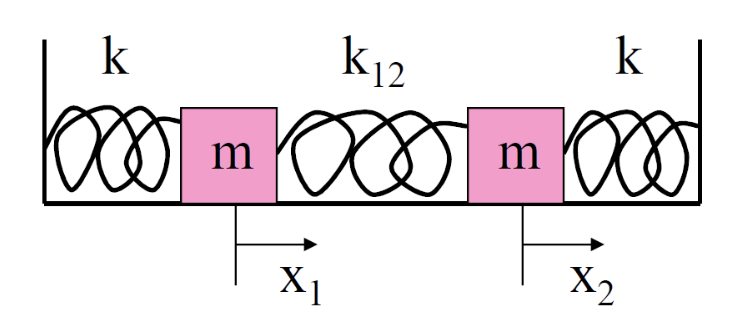
\includegraphics[scale=0.5]{Lecture-10/w10-img1.png}
\end{center}
A system of two coupled harmonic oscillators has spring constants $k$ (left spring), $k_{12}$ (middle spring) and $k$ (right spring). The displacements of the blocks are measured from equilibrium. The forces on the blocks are therefore given by:
\[F_1 = -kx_1 - k_{12}(x_1 - x_2)\]
\[F_2 = -kx_2 - k_{12}(x_2 - x_1)\]
The Lagrangian formulation gives the same result; see worksheet!
\end{document}